%%%%%%%%%%%%%%%%%%%%%%%%%%%%%%%%%%%%%%%%%%%%%%%%%%%%%%%%%%%%%%%%%%%%%%%%%%%%%%%%	
\section{主要工作}

%%%%%%%%%%%%%%%%%%%%%%%%%%%%%%%%%%%%%%%%	
\subsection{概述}

\begin{frame}{工作概述}
  % \fig{width = 0.75\textwidth}{figures/thesis-proposal-3d-framework-allinone.pdf}
  % {数据一致性保障技术研究框架及主要工作: VPC + 2AM + RVSI.}

  \begin{figure}[h!]
    \centering
    \begin{adjustbox}{max totalsize = {0.95\textwidth}{0.75\textheight}, center}
      % allinone: vpc + 2am + rvsi
% with overlays

\begin{tikzpicture}[x = 0.5cm, y = 0.5cm, z = 0.3cm, >=stealth, font = \LARGE]

\only<1->{
\begin{scope}[axesfont/.style = {font = \LARGE}, axesline/.style = {->, line width = 2}, 
  tickline/.style = {line width = 2}, tickfont/.style = {font = \LARGE}]

% the origin
\node[fill = brown, circle] at (0,0,0) {};
% The axes
\draw[axesline] (xyz cs:x=0) -- (xyz cs:x = 18) node[above, axesfont] {$\textrm{Consistency Models}$};
\draw[axesline] (xyz cs:y=0) -- (xyz cs:y = 14) node[above, axesfont] {$\textrm{Assurance Methods}$};
\draw[axesline] (xyz cs:z=0) -- (xyz cs:z = -18) node[right, axesfont] {$\textrm{Data Types}$};

% The ticks

% ticks for consistency models
\draw[tickline] (6,-3pt) -- (6,3pt) node[below = 6pt, tickfont] {Weak};
\draw[tickline] (12,-3pt) -- (12,3pt) node[below = 6pt, tickfont] {Strong};

% ticks for assurance methods
\draw[tickline] (-3pt,5) -- (3pt,5) node[above = 3pt, tickfont] {Maintain};
\draw[tickline] (-3pt,10) -- (3pt,10) node[above = 3pt, tickfont] {Quantify};

% ticks for data types
\draw[tickline] (xyz cs:y=-0.3pt,z=-6) -- (xyz cs:y=0.3pt,z=-6) node[above = 1pt, tickfont] {Register};
\draw[tickline] (xyz cs:y=-0.3pt,z=-12) -- (xyz cs:y=0.3pt,z=-12) node[above = 1pt, tickfont] {Transaction};
\end{scope}
}
%%%%%%%%%% for VPC: register + weak (pram) + quantify (verify)
\only<2>{
  \begin{scope}[line/.style = {line width = 3, dashed, brown}]
	\draw[line]
	  (xyz cs:z = -6) coordinate (z) --
	  (xyz cs:y = 10, z = -6) coordinate (yz) --
	  (xyz cs:x = 0, y = 10, z = 0) coordinate (y) --
	  (xyz cs:x = 6, y = 10) coordinate (xy) --
	  (xyz cs:x = 6, y = 10, z = -6) coordinate (xyz) --
	  (xyz cs:x = 6, z = -6) coordinate (xz) -- cycle;
	\draw[line] (yz) -- (xyz);
	\draw[line] (xy) -- (6,0) -- (xz);
	
    % Dots and labels for P, Q
    \node[fill = brown, circle, inner sep = 5pt, label = {[brown, font = \huge] 0: (\textbf{1.}
  register + pram + verify)}] at (xyz) {};
  \end{scope}
}
%%%%%%%%%% for 2AM
\only<3>{

  \begin{scope}[line/.style = {dashed, line width = 3, blue}]
	\draw[line]
	  (xyz cs:z = -6) coordinate (z) --
	  (xyz cs:y = 5, z = -6) coordinate (yz) --
	  (xyz cs:y = 5) coordinate (y) --
	  (xyz cs:x = 12, y = 5) coordinate (xy) --
	  (xyz cs:x = 12, y = 5, z = -6) coordinate (xyz) --
	  (xyz cs:x = 12, z = -6) coordinate (xz) -- cycle;
	\draw[line] (yz) -- (xyz);
	\draw[line] (xy) -- (12,0) -- (xz);
	
    \node (case-maintain) [fill = blue, circle, inner sep = 5pt, label = {[blue, font = \huge] 90:
    $\qquad \qquad$ (\textbf{2.1} register + atomicity + maintain)}] at (xyz) {};
	
	\draw[line]
	  (xyz cs:z = -6) coordinate (z) --
	  (xyz cs:y = 10, z = -6) coordinate (yz) --
	  (xyz cs:y = 10) coordinate (y) --
	  (xyz cs:x = 12, y = 10) coordinate (xy-am) --
	  (xyz cs:x = 12, y = 10, z = -6) coordinate (xyz) --
	  (xyz cs:x = 12, y = 5, z = -6);
	\draw[line] (yz) --  (xyz);
	\draw[line] (xy-am) -- (12,0) -- (xz);

    \node (case-quantify) [fill = blue, circle, inner sep = 5pt, label = {[blue, font = \huge] 90:
    $\qquad \qquad$ (\textbf{2.2} register + atomicity + quantify)}] at (xyz) {};
  \end{scope}
  }
    % backgroud for case 2.1 and case 2.2
    \begin{pgfonlayer}{background}
      \only<3>{
      \node (case-2am) [fit = (case-maintain) (case-quantify), inner sep = 5pt, ellipse, fill =
      blue!20] {};
    }
    \end{pgfonlayer}


%%%%%%%%%% for RVSI
\only<4>{
  \begin{scope}[line/.style = {dashed, line width = 3, teal}]
      \draw[line]
      (xyz cs:z=-12) coordinate (z) --
      (xyz cs:y=5, z=-12) coordinate (yz) --
      (xyz cs:y=5) coordinate (y) --
      (xyz cs:x=12, y=5) coordinate (xy) --
      (xyz cs:x=12, y=5, z=-12) coordinate (xyz) --
      (xyz cs:x=12, z=-12) coordinate (xz) -- cycle;

      \path[draw, line] (xy) to (xyz cs:x=12) coordinate (x) to (xz);
      \draw[line] (yz) to (xyz);

      \node (rvsi-maintain) [fill = teal, circle, inner sep = 5pt, label = {[above right, teal, font
      = \huge] 0: (\textbf{3.} transaction + SI + maintain)}] at (xyz) {};
	\end{scope}
  }
\end{tikzpicture}


    \end{adjustbox}
    \caption{分布数据一致性及保障技术研究: 
      \only<2->{\textcolor{brown}{VPC}} \only<3->{\textcolor{blue}{ + 
      2AM}} \only<4->{\textcolor{teal}{ + RVSI}}.}
  \end{figure}
\end{frame}
%%%%%%%%%%%%%%%%%%%%%%%%%%%%%%%%%%%%%%%%	
\subsection{VPC: Pipelined-RAM 一致性验证}

\begin{frame}{在研究框架中的位置}
  \fig{width = 0.80\textwidth}{figures/thesis-proposal-3d-framework-vpc.pdf}
  {VPC --- Pipelined-RAM (PRAM) 一致性验证.}
\end{frame}
  

\begin{frame}{研究动机}
  \question{问题: 为什么要验证 Pipelined-RAM (PRAM) 一致性?}
  \vspace{0.50cm}

  \begin{description}
    \setlength{\itemsep}{5pt}
    \item[验证:] 用户需确认存储系统提供了其所声称的数据一致性 \citeinbeamer{Golab}{PODC}{11} 
      \citeinbeamer{Facebook}{SOSP}{15}
      \begin{itemize}
        \item 商用存储系统对于用户是黑盒
        \item 后验分析系统执行
        \item SLA 服务补偿 \citeinbeamer{Amazon}{SOSP}{07}
      \end{itemize}
    \item[PRAM:] 存储系统常提供``会话'' (session) 一致性 
      \citeinbeamer{Saito}{CSUR}{05} \citeinbeamer{Terry}{CACM}{13}
      \begin{itemize}
	\item 包含了弱一致性的诸多变体 
	\item 近似于 PRAM 一致性 \citeinbeamer{Bailis}{VLDB}{13} 
      \end{itemize}
  \end{description}
\end{frame}


\begin{frame}{VPC 问题定义}
  \begin{cdefinition}[VPC: Verifying PRAM Consistency]
    VPC 判定问题:
    \begin{description}
      \item[实例:]
	\begin{itemize}
	  \item 系统执行 (execution $e$; 即, 读写操作序列)
	  \item PRAM 一致性模型 ($\mathcal{C}$)
	\end{itemize}
      \item[问题:]
        \begin{itemize}
          \item 该执行是否满足 PRAM 一致性模型 ($e \in \mathcal{C} \Rightarrow \set{0,1}$)?
        \end{itemize}
    \end{description}    
  \end{cdefinition}
\end{frame}


\begin{frame}{对VPC 问题的系统性研究}
  %%%%%%%%%%%% table: variants of VPC %%%%%%%%%%
  \begin{table}[!t]
    \centering
    \begin{tabular}{|c|c|c|}
      \hline
      & \it (S)ingle variable  & \it (M)ultiple variables
      \\ \hline
      \it write (D)uplicate values &
      \innercell{c}{VPC-SD \\ (NPC) $\textcolor{red}{[\ast]}$} &
      \innercell{c}{VPC-MD \\ (NPC) $\textcolor{red}{[\ast]}$}
      \\ \hline
      \it write (U)nique value &
      \innercell{c}{VPC-SU \\ (P) \citeinbeamer{Golab}{PODC}{11}} &
      \innercell{c}{VPC-MU \\ (P) $\textcolor{red}{[\ast]}$}
      \\ \hline
    \end{tabular}
    \caption{VPC 问题的四种变体 (按``执行''的类型) 及验证复杂性结果 ($\textcolor{red}{[\ast]}: 
    \textrm{new results}$).}
  \end{table}

  \begin{center}
    \textcolor{blue}{论文状态: TPDS'15 录取}
  \end{center}
\end{frame}
%%%%%%%%%%%%%%%%%%%%%%%%%%%%%%%%%%%%%%%%	
\subsection{2AM: Atomicity 一致性维护与量化}


\begin{frame}{在研究框架中的位置}
  \fig{width = 0.80\textwidth}{figures/thesis-proposal-3d-framework-2am}
  {2AM --- Atomicity 一致性维护与量化.}
\end{frame}


\begin{frame}{研究动机}
  \question{问题: 为什么要提出 2-atomicity 一致性?}
  \vspace{0.30cm}

  ``数据一致性/访问延迟'' PACELC 权衡 \citeinbeamer{Abadi}{IEEE Computer}{12}:

  \fignocaption{width = 0.40\textwidth}{figures/stronger-consistency-tradeoff.pdf}

  % \begin{quote}
  %   ``As soon as a distributed storage system replicates data, a \textcolor{brown}{tradeoff 
  %   between consistency and latency} arises.''
  % \end{quote}

  为保证低延迟, 采用较弱一致性:
  \begin{quote}
    ``{\small 100ms of additional latency = 1\% drop in sales}'' \hfill -- {\scriptsize 
      \textcolor{blue}{[Amazon'06]}} \end{quote}

  {\small
  \begin{table}
    \begin{tabular}{c|c}
      \hline
      \textcolor{blue}{\bf 系统} & \textcolor{blue}{\bf 一致性}		\\ \hline
      Dynamo@Amazon & eventual consistency \\ \hline
      Tao@Facebook & read-after-write \\ \hline
      PNUTS@Yahoo! & cache consistency \\ \hline
    \end{tabular}
  \end{table}
  }
\end{frame}


\begin{frame}{2-atomicity 一致性}
  % \begin{cdefinition}[``近乎强''一致性]
  %   对某特定强一致性的弱化: \begin{itemize}
  %     \item (版本) 允许读陈旧值,但陈旧度有限
  %     \item (概率) 读到陈旧值的概率很小
  %   \end{itemize}
  % \end{cdefinition}

  \begin{center}
    \answer{2AM: 在保证低延迟的情况下获得尽可能强的数据一致性.}
  \end{center}

  \begin{cdefinition}[2-atomicity 一致性]
    \begin{description}
      \item[低延迟:] 读操作只需一轮网络通信
      \item[尽可能强:] 对 atomicity (最强) 的弱化
    \begin{itemize}
      \item (版本) 允许读陈旧值,且\textcolor{red}{陈旧度 $k \le 2$}
      \item (概率) \textcolor{red}{$\mathbb{P}(k = 2)$ 很小}
    \end{itemize}
    \end{description}
  \end{cdefinition}
\end{frame}


\begin{frame}{2AM 维护算法}
  2AM (单写多读) 维护算法: \textcolor{red}{读} (写)只需一轮网络通信

  \fig{width = 0.80\textwidth}{figures/atomicity-2am-read-compare.pdf}
  {经典 atomicity 算法中, 读操作需两轮网络通信 \citeinbeamer{ABD}{JACM}{95} 
  \citeinbeamer{Dutta}{PODC}{04}. 2AM 算法中, 读操作只需一轮网络通信: 
读取半数以上副本节点, 返回最新值.}
\end{frame}


\begin{frame}{2AM 量化分析}
  \question{问题: 2AM 算法在多大程度上违反了 atomicity?}
  \vspace{0.30cm}

  \begin{itemize}
    \setlength{\itemsep}{8pt}
    \item 充要条件: ONI (old-new inversion)
      \fignocaption{width = 0.45\textwidth}{figures/2atomicity-case.pdf}
    \item 2AM 量化分析: 计算 $\mathbb{P}(\textrm{ONI})$, 其值越小越好
      \begin{enumerate}
        \setlength{\itemsep}{3pt}
        \item $\textrm{ONI} \triangleq \textrm{CP} \cap \textrm{RWP}$
        \item 排队论建模, 计算 $\mathbb{P}(\textrm{CP})$ \item 带时间的球盒模型, 计算 
          $\mathbb{P}(\textrm{RWP|CP})$
        % \item 实验统计 $\mathbb{P}(\textrm{CP})$, $\mathbb{P}(\textrm{RWP|CP})$ 与 
        % $\mathbb{P}(\textrm{ONI})$, 以作对照
      \end{enumerate}
  \end{itemize}
\end{frame}


\begin{frame}{2AM 量化分析}
  \begin{itemize}
    \item 公式推导:
      \begin{figure}[h]
        \centering
        \subfloat{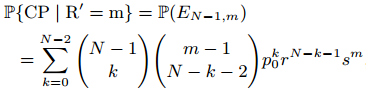
\includegraphics[width = 0.30\textwidth]{figures/cp.png}}
        \qquad
        \subfloat{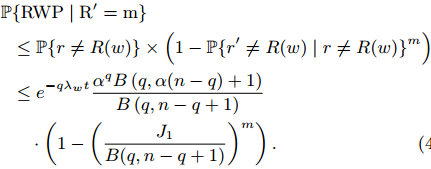
\includegraphics[width = 0.40\textwidth]{figures/rwp.png}}
      \end{figure}
    \item 数值结果 (左一) 与实验结果 (右二): \begin{figure}[h]
        \centering
        \subfloat{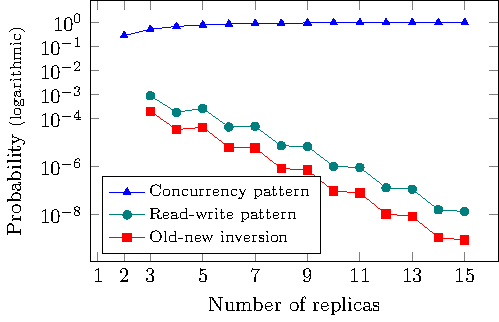
\includegraphics[width = 0.30\textwidth]{figures/oni-pgfplot.pdf}}
        \quad
        \subfloat{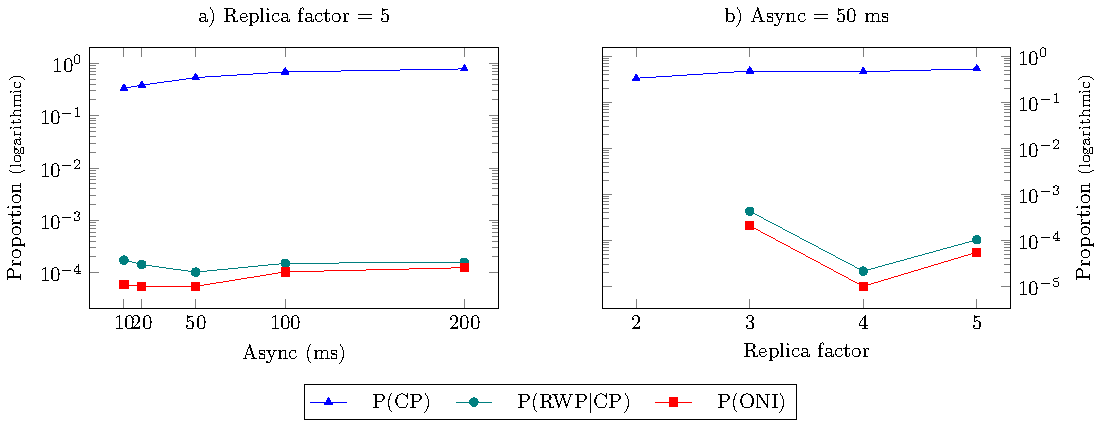
\includegraphics[width = 0.50\textwidth]{figures/experiment-oni-pgfplot.pdf}}
      \end{figure}
  \end{itemize}
  \begin{center}
    \textcolor{blue}{论文状态: TC 在审}
  \end{center}
\end{frame}
%%%%%%%%%%%%%%%%%%%%%%%%%%%%%%%%%%%%%%%%	
\subsection{RVSI: Snapshot Isolation 一致性弱化与维护}

\begin{frame}{在研究框架中的位置}
  \fig{width = 0.80\textwidth}{figures/thesis-proposal-3d-framework-rvsi.pdf}
  {RVSI --- Snapshot Isolation 一致性弱化与维护}
\end{frame}


\begin{frame}{研究动机}
  \question{问题: 为什么要提出 RVSI 一致性?}
  \vspace{0.30cm}

  \begin{description}
    \setlength{\itemsep}{5pt}
    \item[分布式事务:] 
      \begin{itemize}
        \item ``all-or-none'' 语义
        \item 受到分布式存储系统的关注 \citeinbeamer{Cassandra}{CASSANDRA-ISSUE-7056}{14}
      \end{itemize}
    \item[弱一致性:] 
      \begin{itemize}
        \item PCSI \citeinbeamer{Elnikety}{SRDS}{05} \textcolor{red}{SI} \citeinbeamer{Lin}{TODS}{09} \\
          PSI \citeinbeamer{Sovran}{SOSP}{11} NMSI \citeinbeamer{Ardekani}{SRDS}{13} 
        \end{itemize}
    \pause
    \item[\question{异常控制}:]
      \begin{itemize}
        \item 容忍``有限度的''异常 \citeinbeamer{Yu}{TOCS}{02}
      \end{itemize}
    \item[\question{可定制}:] 
      \begin{itemize}
        \item 不同应用对一致性需求不同 \citeinbeamer{Terry}{CACM}{13}
        \item 运行时决定 \citeinbeamer{Terry}{SOSP\&TR}{13}
      \end{itemize}
  \end{description}
 
  \pause
  \vspace{0.30cm}
  \textcolor{red}{RVSI (Relaxed Version Snapshot Isolation):}
  \begin{enumerate}
    \item 支持可定制一致性 
    \item 提供``有限度的''异常控制 
    \item 支持高效的分布式实现
  \end{enumerate}
\end{frame}


\begin{frame}{RVSI 定义}
  RVSI 定义原则:
  \begin{itemize}
    \item 参数 $k_1, k_2, k_3$ 控制``异常''程度
    \item $\text{RC} \supset \text{RVSI}(k_1, k_2, k_3) \supset \text{SI}$
    \item $\text{RVSI}(\infty,\infty,\infty) = \text{RC}; \qquad \text{RVSI}(1,0,\ast) = \text{SI}$
  \end{itemize}

  \begin{cdefinition}[RVSI: Relaxed Version Snapshot Isolation]
    \begin{description}
      \item[单变量读 $\texttt{read}(x)$:] \hfill 
        \begin{enumerate}
          \item 允许读 $\le k_1$ 陈旧值
          \item 允许读 $\le k_2$ 并发更新
        \end{enumerate}
      \item[多变量读 $\texttt{read}(x), \texttt{read}{(y)}$:] \hfill
        \begin{enumerate}
          \setcounter{enumi}{2}
          \item $\textsf{dist}(x,y) \le k_3$
        \end{enumerate}
    \end{description}
  \end{cdefinition}
\end{frame}


\begin{frame}{RVSI 维护算法}
  \[
    \textcolor{blue}{\text{RC} \supset \text{RVSI}(k_1, k_2, k_3) \supset \text{SI}}
  \]

  \vspace{0.10cm}

  RVSI 维护算法:
  \begin{itemize}
    \item 以分布式 RC 和 SI 协议 为基础
    \item 事务执行时, 添加 RVSI ``版本约束'' ($k_1, k_2, k_3$ 相关)
    \item 事务提交时, 检查 RVSI ``版本约束''
  \end{itemize}

  \pause

  \vspace{0.30cm}
  RVSI 实验:
  \begin{itemize}
    \item \textcolor{blue}{Chameleon:} a distributed, partitioned, replicated, transactional key-value store
    \item Amazon 云端部署 (计划中)
  \end{itemize}

  \textcolor{red}{\small \url{https://github.com/hengxin/chameleon-transactional-kvstore}}

  \begin{center}
    \textcolor{blue}{论文状态: 准备中; 计划投稿 SRDS'16}
  \end{center}
\end{frame}
